\chapter{Probabilistic model checking}
Discrete-time Markov chain is a formalism often used to model stochastic population process. In this
chapter, we present essential concepts on probabilistic model checking, including probabilistic
models and properties. We also briefly present a general deterministic model checking algorithm for
a specific temporal logic, namely Probabilistic Computational Tree Logic (or PCTL in short). Due to
the state space explosion, applying a deterministic model checking algorithm is often
computationally expensive. Therefore, we also present a simulation-based model checking, namely
statistical model checking (or SMC in short) for bounded path property. We also introduce
definitions of parametric DTMC and the parameter synthesis problem, and the symbolic computing
approach to verify parametric models.


\section{Markov models}
\subsection{Discrete Time Markov chain}
Markov models are stochastic models evolving in discrete or continuous time, which satisfy the
\textit{memoryless property}. Memoryless property is a property of stochastic processes, which
refers to the independence of the future states of the process on its previously visited states.
Discrete-time Markov chain is a Markov model of discrete state-space and countable (discrete) time. In
a discrete-time Markov chain, times between any state transition are uniform.
\begin{definition}[Discrete Time Markov Chain \cite{baier2008principles}]
      \rm
      A \textit{Discrete-time Markov chain} (or DTMC in short) $\mathcal{M}$ is a tuple
      $(S,\mathbf{P}, \iota_{init}, AP, L)$, in which
      \begin{itemize}
            \item $S$ is a countable, non-emty set of \textit{states}
            \item $\mathbf{P}:S\times S \rightarrow [0,1]$ is the \textit{transition probability}
                  function such that
                  \begin{align*}
                        \forall s \in S : \sum_{s'\in S}\mathbf{P}(s, s') = 1
                  \end{align*}
            \item $\iota_{init}: S \rightarrow [0,1]$ is the \textit{initial distribution} such that
                  \begin{align*}
                        \sum_{s\in S} \iota_{init}(s) = 1
                  \end{align*}
            \item $AP$ is a set of \textit{atomic propositions}.
            \item $L: S \rightarrow 2^{AP}$ is the labelling function on states.
      \end{itemize}
\end{definition}

\begin{example}[Knuth-Yao die]
      \rm
      Knuth and Yao \cite{knuth1976complexity} introduced an algorithm to simulate a fair dice by a
      fair coin. The algorithm terminates returning one among six possible outcomes of a die tossing
      (from one to six). We formalize the algorithm by a DTMC with 6 BSCCs. Each of the 6 BSCCs
      represents a possible outcome of a die tossing. The probabilities of reaching each BSCC among
      the six is $1/6$.
      \begin{figure}[H]
            \centering
            \begin{forest}
                  for tree={
                  edge = {->},
                  circle,
                  minimum size=1cm,
                  inner sep=0pt,
                  l+=15pt,
                  draw,
                  math content,
                  tier/.wrap pgfmath arg={tier #1}{level()},
                  anchor=center
                  },
                  [S_0, initial
                  [S_1, edge label={node[midway, above left]{$\frac{1}{2}$}}, name=s1
                  [S_3, edge label={node[midway, below right]{$\frac{1}{2}$}}, name=s3
                  [\textbf{1}, edge label={node[midway, left]{$\frac{1}{2}$}}, accepting,]
                  ]
                  [S_4, edge label={node[midway, above right]{$\frac{1}{2}$}},
                  [\textbf{2}, edge label={node[midway, above left]{$\frac{1}{2}$}}, accepting,],
                  [\textbf{3}, edge label={node[midway, above right]{$\frac{1}{2}$}}, accepting]
                  ]
                  ]
                  [S_2, edge label={node[midway, above right]{$\frac{1}{2}$}}, name=s2
                  [S_5, edge label={node[midway, below right]{$\frac{1}{2}$}}, name=s5
                  [\textbf{4}, edge label={node[midway, left]{$\frac{1}{2}$}}, accepting,]
                  ]
                  [S_6, edge label={node[midway, above right]{$\frac{1}{2}$}}
                        [\textbf{5}, edge label={node[midway, above left]{$\frac{1}{2}$}}, accepting,]
                        [\textbf{6}, edge label={node[midway, above right]{$\frac{1}{2}$}}, accepting,]
                  ]
                  ]
                  ]
                  \draw[->] (s3) to [bend left] node[above left]{$\frac{1}{2}$} (s1);
                  \draw[->] (s5) to [bend left] node[above left]{$\frac{1}{2}$} (s2);
            \end{forest}
            \caption{DTMC model of Knuth-Yao algorithm. The accepting states $1$ to $6$ represent a face of a fair die.}
            \label{fig:knuth-die}
      \end{figure}
\end{example}

\begin{definition}[Strongly Connected Component]
      \rm
      Let $\mathcal{M}=(S,\mathbf{P}, \iota_{init}, AP,L)$ be a DTMC. A subset $S'\subset S$ is
      \textit{strongly connected} if and only if for every pair $s_1,s_2\in S'$ there is a path
      between $s_1$ and $s_2$ which consists of only states in $S'$. If $S'$ has no superset
      $S''\subseteq S$, such that $S''$ is strongly connected, then $S'$ is a \textit{Strongly
            Connected Component}, or \textit{SCC} in short.
\end{definition}

\begin{definition}[Bottom Strongly Connected Component]
      \rm
      Let $\mathcal{M}=(S,\mathbf{P}, \iota_{init}, AP,L)$ be a DTMC and $S'\in S$ a Strongly
      Connected Component. $S'$ is also a \textit{Bottom Strongly Connected Component} (or
      \textit{BSCC} in short), if and only if there exist no state $s \in S\backslash S'$ that is reachable
      from any state in $S'$. If $|S'|=1$ then $S'$ is a \textit{trivial BSCC}. We denote
      $BSCC(\mathcal{M})\in S$ is the set of all BSCCs of $\mathcal{M}$.
\end{definition}

\noindent Intuitively, BSCCs are arbsobing; once a path in a DTMC reaches a state in a BSCC, it visits  all
states in the BSCC infinitely often. It is proven by \cite{baier2008principles} that any run on a
DTMC $\mathcal{M}$ ends in $BSCC(\mathcal{M})$ almost surely.
\begin{theorem}[Long-run theorem]
      \rm
      Let $\mathcal{M}=(S,\mathbf{P}, \iota_{init}, AP,L)$ be a DTMC. Let $BSCC(\mathcal{M})$ be the
      set of all BSCCs of $\mathcal{M}$. Then, the probability of reaching a BSCC and visit all of
      its states infinitely often is equal to 1. Formally
      \begin{align*}
            Pr(\Diamond BSCC(\mathcal{M})) = 1
      \end{align*}
\end{theorem}

\noindent In this thesis, we use the experiment data as the \textit{steady-state distribution} of a
DTMC.
\begin{theorem}[Steady-state distribution]
      \rm
      Let $\mathcal{M}=(S,\mathbf{P}, \iota_{init}, AP,L)$ be a DTMC and a vector $\nu_t \in
            [0,1]^{|S|}$ be a transient state distribution at time $t\in\mathbb{N}$ defined by
      \begin{align*}
            \nu_t = (Pr(X_t=s_1),\ldots,Pr(X_t=s_{|S|})) \quad s_1,\ldots,s_{|S|} \in S
      \end{align*}
      A transient state distribution $\nu$ of $\mathcal{M}$ is a \textit{steady-state distribution}
      of $\mathcal{M}$ if and only if
      \begin{align*}
            t\rightarrow \infty: \nu_t = \nu_t P
      \end{align*}
\end{theorem}
\noindent As a result from long-run theorem, we have the following lemma regarding the existence of
the steady state distribution in DTMC with BSCC(s)
\begin{lemma}[]
      \rm
      Let $\mathcal{M}=(S,\mathbf{P}, \iota_{init}, AP,L)$ be a DTMC and $BSCC(\mathcal{M})$ be the
      set of all BSCCs of $\mathcal{M}$. If $BSCC(\mathcal{M})\neq \emptyset$ then there exists a
      steady-state distribution $\nu = (Pr(X=s_1),\ldots,Pr(X=s_{|S|}))$, such that
      \begin{align*}
            \forall i: 1 \leq i \leq |S|: P(X=s_i) \neq 0
      \end{align*}
      if and only if
      \begin{align*}
            s_i \in BSCC(\mathcal{M})
      \end{align*}
\end{lemma}


\subsection{Continuous-time Markov chain}
The discrete-time memoryless property can also be extended into continuous-time memoryless property.
Continuous-time Markov chain is often used to model a system in which times between transitions
vary and are real numbers.
\begin{definition}[Continuous-time Markov chain \cite{katoen2001faster}]
      A \textit{Continuous-time Markov chain} (or CTMC in short) $\mathcal{C}$ is a tuple
      $(S,\mathbf{P}, \mathbf{R}, \iota_{init}, AP, L)$, where
      \begin{itemize}
            \item $S$ is a countable, non-emty set of \textit{states}
            \item $\mathbf{R}:S\times S \rightarrow \mathbb{R}_{>0}$ is the \textit{rate matrix}.
            \item $\iota_{init}: S \rightarrow [0,1]$ is the \textit{initial distribution} such that
                  \begin{align*}
                        \sum_{s\in S}\iota_{init}(s) = 1
                  \end{align*}
            \item $AP$ is a set of \textit{atomic propositions}
            \item $L: S \rightarrow 2^{AP}$ is the labelling function on states.
      \end{itemize}
\end{definition}

\begin{example}[CTMC]
      We give an example of a CTMC $\mathcal{C}=(S,\mathbf{R}, \iota_{init}, AP, L)$, where
      \begin{itemize}
            \item State set $S=\{S_0, S_1, S_2\}$
            \item Initial state $\iota_{init} = \{S_0\}$
            \item Transition rate matrix
                  $$
                        \mathbf{R} = \begin{bmatrix}
                              0           & 2 & 0           \\
                              \frac{4}{3} & 0 & \frac{8}{3} \\
                              0           & 3 & 0
                        \end{bmatrix}
                  $$
      \end{itemize}
      \begin{figure}[H]
            \centering
            \begin{tikzpicture}[->, >=stealth', auto, semithick, node distance=3cm]
                  \tikzstyle{every state}=[fill=white,draw=black,thick,text=black]
                  \node[state, initial]    (S0)                   {$S_0$};
                  \node[state]             (S1)[right of=S0]      {$S_1$};
                  \node[state]             (S2)[right of=S1]      {$S_2$};
                  \path
                  (S0)
                  edge [bend left=20] node{$2$} (S1)
                  (S1)
                  edge [bend left=20] node{$\frac{8}{3}$} (S2)
                  edge [bend left=20] node{$\frac{4}{3}$} (S0)
                  (S2)
                  edge [bend left=20] node{$3$} (S1);
            \end{tikzpicture}
            \label{fig:ctmc}
            \caption{An example of a CTMC with 3 states.}
      \end{figure}
\end{example}

\begin{definition}[Exit rate \cite{katoen2001faster}]
      \rm
      Let $\mathcal{C} = (S,\mathbf{R}, \iota_{init}, AP, L)$ be a CTMC. We define the \textit{exit
            rate} $\mathbf{E}(s), s\in S$ as the row sum of the rate matrix $\mathbf{R}$
      \begin{align*}
            \mathbf{E}(s) = \sum_{s'\in S} \mathbf{R}(s, s')
      \end{align*}
\end{definition}

CTMC is a solid formalism to model systems concerning real-time properties. In this thesis, we
transform CTMCs into DTMCs through a process of \textit{uniformization} \cite{katoen2001faster}.
Uniformization discretizes a CTMC by transforming it in to a CTMC which has uniform exit rates among
states, so that we can approximate the uniformized CTMC using a DTMC by removing the exit rates, and
modelling times between transitions by a Poisson process with rate equal to the chosen
uniformization constant. Katoen \cite{katoen2001faster} shows that the uniformization of CTMC
preserves the transient probabilities. Baier \cite{baier2002simulation} proved that the time-bounded
until formulas remain unaffected as we transform a CTMC to its equivalent uniformized form. Through
uniformization, we can check the time-bounded reachability property. Furthermore, transforming a
CTMC to an equivalent DTMC allows us to obtain a symbolic form of the PCTL formula, thus enabling a
more efficient evaluation of properties.

\begin{definition}[CTMC uniformization \cite{katoen2001faster}]
      \rm
      Let $\mathcal{C} = (S,\mathbf{R}, \iota_{init}, AP, L)$ be a CTMC with exit rate $E(s), s\in S$. We
      define the \textit{uniformization rate} $r$ such that
      \begin{align*}
            \forall s\in S: r \geq \mathbf{E}(s), r\in\mathbb{R}_{>0}
      \end{align*}
      The \textit{uniformized CTMC} $unif(r, \mathcal{C})=(S, \bar{\mathbf{R}}, \iota_{init}, AP, L )$ such that
      \begin{align*}
            \forall s, s'\in S & : \bar{\mathbf{R}}(s,s')=
            \begin{cases}
                  \frac{\mathbf{R}(s,s')}{r}                               & \text{if $s \neq s'$} \\ \quad \\
                  \frac{\mathbf{R}(s,s')}{r} + 1 - \frac{\mathbf{E}(s)}{r} & \text{if $s = s'$}
            \end{cases}
      \end{align*}
\end{definition}

\begin{example}[Uniformized CTMC]
      After uniformizing the CTMC in Figure \ref{fig:ctmc} by uniformization rate $r=4$, we obtain the followig DTMC
      \begin{figure}[H]
            \centering
            \begin{tikzpicture}[->, >=stealth', auto, semithick, node distance=3cm]
                  \tikzstyle{every state}=[fill=white,draw=black,thick,text=black]
                  \node[state, initial]    (S0)            {$S_0$};
                  \node[state, ]    (S1)[right of=S0]      {$S_1$};
                  \node[state, ]    (S2)[right of=S1]      {$S_2$};
                  \path
                  (S0)
                  edge [bend left=20] node{$\frac{1}{2}$} (S1)
                  (S1)
                  edge [bend left=20] node{$\frac{2}{3}$} (S2)
                  edge [bend left=20] node{$\frac{1}{3}$} (S0)
                  (S2)
                  edge [bend left=20] node{$\frac{3}{4}$} (S1);
            \end{tikzpicture}
            \caption{Uniformized DTMC}
            \label{fig:uniformized-ctmc}
      \end{figure}
\end{example}


\section{Property specification}
\subsection{Probabilistic Computational Tree Logic}
Model checking verifies a system \textit{(model)} against a property of interest. We
formalize a property by a \textit{temporal logic}, specifically \textit{Probabilistic Computational
      Tree Logic} (or \textit{PCTL}). Firstly introduced by Hansson et al. \cite{hansson1994logic}, PCTL
is widely used in model checking of discrete-time stochastic models and supported by
probabilistic model checking tools Storm \cite{dehnert2017storm}, and PRISM \cite{kwiatkowska2011prism}.
\begin{definition}[PCTL \cite{baier2008principles}]
      \rm
      The syntax of PCTL consists of state formulas and path formulas.
      \begin{itemize}
            \item State formulas are defined over $AP$
                  \begin{align*}
                        \Phi & ::= \text{true} \;|\; a \;|\; \Phi \;|\; \Phi_1 \wedge \Phi_2 \;|\; \Phi_1 \vee \Phi_2 \;|\;  P_{J}(\phi)
                  \end{align*}
                  where $a\in AP$, $\phi$ is a path formula, and $J\subseteq[0,1]$ is an interval.
            \item Path formulas
                  \begin{align*}
                        \phi & ::= \bigcirc \Phi \;|\; \Phi_1 \mathsf{U} \Phi_2 \;|\; \Phi_1 \mathsf{U}^{\leq n} \Phi_2
                  \end{align*}
                  where $\Phi,\Phi_1,\Phi_2$ are state formulas, and $n\in \mathbb{N}$.
      \end{itemize}
\end{definition}

\begin{example}
      Given the DTMC as in Figure \ref{fig:knuth-die}. The probability that the simulation eventually ends with the outcome "one dot" is equal to $\frac{1}{6}$:
      \begin{align*}
            P_{=\frac{1}{6}}(\Diamond 1)
      \end{align*}
\end{example}

\noindent  In a DTMC, a PCTL state formula is verified at each state, while a PCTL path formula is
verified through a trace from an execution path. The algorithm to model check DTMC against PCTL
properties is described in detail in Katoen \cite{baier2008principles}. Given a DTMC $\mathcal{M}$
and a PCTL property $\Phi$, general algorithm for checking $\mathcal{M}\models\Phi$ has time
complexity polynomial to $|\mathcal{M}|$ and linear to $|\Phi|$.
\begin{theorem}[Complexity of checking a DTMC against a PCTL formula \cite{katoen2013model}]
      For finite DTMC $\mathcal{M}$ and PCTL state-formula $\Phi$,the PCTL model-checking problem
      can be solved in time
      \begin{align*}
            \mathcal{O}(poly(size(D)\cdot n_{max} \cdot |\Phi|))
      \end{align*}
      where
      \begin{align*}
            n_{max} =
            \begin{cases}
                  max(n | (\Psi_1 \mathsf{U}^{\leq n} \Psi_2) \quad\text{occurs in}\quad \Phi) \\
                  1 \text{ if $\Phi$ contains no bounded until property}
            \end{cases}
      \end{align*}
\end{theorem}

\subsection{State explosion problem}
The \textit{state-explosion problem} occurs when the size of a model state space grows exponentially
as the number of state variables in the system increases \cite{clarke2011model}. As a finite-state
abstraction of a system, each state in a model consists of state variables, which encode a property
of the system it models. However, due to the combinatorial explosion, the state-space grows
exponentially in size. For example, consider a distributed software system, in which a
\textit{global state} is a composition of
\begin{enumerate}
      \item $N$ 8-bit integer variables, and
      \item $M$ communication channels of capacity $Q$.
\end{enumerate}
The total number of global states is $2^{8N}Q^M$. The size of state-space grows exponentially as we
add new variables and communication channels. As discussed before, the complexity of model
checking a PCTL property against a DTMC model is polynomial to the DTMC's state-space. However, the
state-explosion problem renders model checking computationally expensive. One possible way to cope
with the state-explosion problem and to reduce the computational cost is to use \textit{statistical
      model checking}.

\section{Statistical model checking}
Statistical model checking is a simulation-based approach to model check a stochastic model
$\mathcal{D}$ against a PCTL property $\Phi$. The essential concept of probabilistic model checking
is to simulate a number of traces from $\mathcal{M}$, monitor if each trace satisfies $\Phi$, then
estimate probability $P(\mathcal{M}\models\Phi)$ by a statistical inference \cite{agha2018survey}.\\
Given a stochastic model $\mathcal{M}$ and a property $\Phi$, statistical model checking solves the
\textit{qualitative} and \textit{quantitative}
problem\footnote{\url{https://www-verimag.imag.fr/Statistical-Model-Checking-814.html\#nb3}}:
\begin{enumerate}
      \item \textbf{Quantitative}: Estimate the probability $p = Pr(\mathcal{M}\models\Phi)$. In
            other words, it checks $\mathcal{M}$ the property \begin{align*} P_{=?}(\Phi)
            \end{align*}
      \item \textbf{Qualitative}: Decide if $p = Pr(\mathcal{M}\models\Phi)$ is greater or less than
            a threshold $\epsilon$. In other words, it checks $\mathcal{M}$ the property
            \begin{align*} P_J(\Phi)
            \end{align*}
            where $J\subseteq[0,1]$ is an interval.
\end{enumerate}

\begin{table}[H]
      \centering
      \begin{tabular}{|l|l|l|}
            \hline
                   & {\color[HTML]{232627} Quantitative} & Qualitative                         \\ \hline
            Input  & \begin{tabular}[c]{@{}l@{}}Model $\mathcal{M}$\\ Property $P_{=?}(\Phi)$\end{tabular}          & \begin{tabular}[c]{@{}l@{}}Model $\mathcal{M}$\\ Property $P_J(\Phi), J\subseteq[0,1]$\end{tabular}          \\ \hline
            Output & $p=P(\mathcal{M}\models\Phi)$       & $P(\mathcal{M}\models\Phi) \in J$ ? \\ \hline
      \end{tabular}
      \caption{Input and output of quantitative and qualitative statistical model checking}
\end{table}



\subsection{Statistical model checking of quantitative properties.}
Given an \textit{approximation parameter} $\epsilon$ and a \textit{confidence parameter}
$\alpha$, we estimate $\hat{p}$ as an estimation of $p$ such that
\begin{align*}
      Pr(|p-\hat{p}| \leq \epsilon) \geq 1 - \alpha
\end{align*}
How many simulations must be performed?  As verifying a simulation trace against a reachability
property $\Phi$ is Bernoulli trial (satisfied or not satisfied), the number of simulation $N$ can be
estimated using different bounds. Chernoff \cite{chernoff2014career} presents Chernoff inequality to
estimate $N$ for Bernoulli trials. Hoeffding \cite{hoeffding1963probability} later extends Chernoff
inequality to general cases.\\
Let $Sat(N)$ be number of satisfying traces in $N$ sampled traces. By applying Chernoff-Hoeffding
inequality we obtain
\begin{align*}
      P(|\frac{Sat(N)}{N}-p| > \epsilon)                                    & \leq 2\exp{\frac{-N\epsilon^2}{4}}     \\
      \llap{$\Leftrightarrow$ \qquad} P[|\frac{Sat(N)}{N}-p| \leq \epsilon] & \geq 1 - 2\exp{\frac{-N\epsilon^2}{4}}
\end{align*}
Replacing $\alpha = 2\exp{\frac{-N\epsilon^2}{4}}$ and $\hat{p}=\frac{Sat(N)}{N}$, we have
\begin{align*}
      P[|\hat{N} - p| \leq \epsilon]                  & \geq 1 - 2\alpha                               \\
      \llap{$\Leftrightarrow$ \qquad \qquad \qquad} N & \geq 4\frac{\ln{\frac{2}{\alpha}}}{\epsilon^2}
\end{align*}
For example, given approximation parameter $\epsilon=0.01$ and confidence parameter $\alpha=0.05$,
we obtain $N\geq 147556$. However, if we want a more precise estimation, for example
$\epsilon=0.005$, then the total number of simulation runs $N\geq 590221$. In other words, the total
number of simulation runs is proportional to the quadratic reciprocal of the approximation parameter
$\epsilon$. The estimation algorithm \textit{Approximate Probabilistic Model Checking} (APMC in
short) is described in detail in \cite{herault2004approximate}.
\begin{algorithm}[H]
      \caption{Statistical Model Checking, APMC method.}
      \label{alg:smc-apmc}
      \footnotesize{
            \hspace*{\algorithmicindent} \textbf{Input:}
            \begin{itemize}[noitemsep,topsep=0pt]
                  \item $\mathcal{D}$: a DTMC
                  \item $\alpha, \epsilon$: confidence level and approximation, respectively.
                  \item $\Phi = P_{=?}(\varphi) $: a PCTL property to be evaluated $\mathcal{D}$
            \end{itemize}
            \hspace*{\algorithmicindent} \textbf{Output:} $\hat{p}$: an estimation of $p$, ($p = Pr(\mathcal{D} \models \varphi)$)
      }
      \begin{algorithmic}[1]
            \Procedure{SMC-APMC}{}
            \State $N \leftarrow 4\frac{\ln{\frac{2}{\alpha}}}{\epsilon^2}$
            \State $A \leftarrow 0$
            \State $i \leftarrow 1$
            \While{$i \leq N$}
            \State Simulate a trace $t$ from $\mathcal{D}$ by discrete-event simulation.
            \If{$t \models \phi$}
            \State $A \leftarrow A + 1$
            \EndIf
            \EndWhile
            \Return $\frac{A}{N}$
            \EndProcedure
      \end{algorithmic}
\end{algorithm}
The Chernoff-Hoeffding gives a lower bound of total simulation runs $N$ to estimate a satisfaction
property with a specific error margin.

\subsection{Statistical model checking of qualitative properties.}
Wald \cite{wald1945sequential} introduces the Sequential Probability Ratio Test (SPRT in short) to
perform hypothesis tests on sequential statistical analysis, in which the sample size $N$ is not
known \textit{a priori}. SPRT updates a cumulative sum and stops when it has enough information to
accept the null hypothesis or alternative hypothesis statistically.\\
Younes \cite{younes2002probabilistic} introduces an application of Wald's SPRT on statistical model
checking. Given a DTMC $\mathcal{D}$ and a PCTL property $\Phi$ with probabilistic bound $\Phi =
      P_J(\varphi)$. Without loss of generality, we asume that $\Phi = P_{\geq p}(\varphi),
      p\in[0,1]$. The SPRT method tests the following null hypothesis and alternative hypothesis with
approximation width $\epsilon$:
\begin{align*}
       & H_0: \hat{p} \geq p + \epsilon \\
       & H_1: \hat{p} < p - \epsilon
\end{align*}
Let $A$ be the set of satisfying traces among total $N$ simulated traces from $\mathcal{D}$. Given
probability of success in a single Bernoulli trial is $p$, we have
\begin{align*}
      P(A | p) = {N \choose A} \cdot p^A(1-p)^{N-A}
\end{align*}
As a new trace $t$ is collected from a simulation run on $\mathcal{D}$, SPRT updates the set of
satisfying traces $A$. It then computes the likelihood ratio based on $A$:
\begin{align*}
      R = \frac{P(A | p + \epsilon)}{P(A | p - \epsilon)}
\end{align*}
Let $\alpha$ and $\beta$ be error of type I and type II, respectively, that is,
\begin{align*}
       & \alpha = Pr(\mathcal{D} \models \Phi | \text{Accept}\quad H_1) \\
       & \beta =  Pr(\mathcal{D} \nvDash \Phi | \text{Accept}\quad H_0)
\end{align*}
We compute bounds for accepting or rejecting null hypothesis
\begin{align*}
      p_0 & = \frac{\beta}{1 - \alpha} \\
      p_1 & = \frac{\alpha}{1 - \beta}
\end{align*}
Wald's sequential probabilistic ratio test allows the algorithm to terminate as soon as simulated
traces reach either of the two bounds $p_0$ or $p_1$.
\begin{algorithm}[H]
      \caption{Statistical Model Checking, SPRT method}
      \label{alg:smc-sprt}
      \footnotesize{
            \hspace*{\algorithmicindent} \textbf{Input:}
            \begin{itemize}[noitemsep,topsep=0pt]
                  \item $\mathcal{D}$: a DTMC
                  \item $\alpha, \beta$: probability of type I and type II error respectively.
                  \item $\epsilon$: approximation width.
                  \item $\Phi = P_{\geq p}(\varphi)$: a PCTL property in $\mathcal{D}$
            \end{itemize}
            \hspace*{\algorithmicindent} \textbf{Output:} $(\mathcal{D} \models \Phi)$ or $(\mathcal{D} \nvDash \Phi)$
      }
      \begin{algorithmic}[1]
            \Procedure{SMC-SPRT}{}
            \State $p_0 = \frac{\beta}{1 - \alpha}$
            \State $p_1 = \frac{\alpha}{1 - \beta}$
            \State $N \leftarrow 0$
            \State $A \leftarrow 0$
            \While{$\texttt{True}$}
            \State Simulate a trace $T$ from $\mathcal{D}$
            \If{$T \models \Phi$}
            \State Append $T$ to $A$
            \EndIf
            \State $R \leftarrow \frac{P(A | p + \delta)}{P(A | p - \delta)}$
            \If{$R \geq p_1$}
            \State Accept $H_1$, return $(\mathcal{D} \nvDash \Phi)$
            \Else
            \If{$R \leq p_0$}
            \State Accept $H_0$, return $(\mathcal{D} \models \Phi)$
            \EndIf
            \EndIf
            \EndWhile
            \EndProcedure
      \end{algorithmic}
\end{algorithm}


\section{Parametric model checking}
\subsection{Parametric discrete-time Markov chain}
In order to generalize the model and encompass the unknown features of the interested system in
DTMC, we introduce \textit{parameters} into transition probabilities. In this thesis we assume that
parameters' domain is $\mathbb{R}$.
\begin{definition}[Rational functions]
      \rm
      Let $\theta=\{x_1,\ldots,x_n\}$ be a variable; let $\mathbf{Pol}[\mathbf{x}]$ be the set of
      all polynomial functions over $\mathbf{x}$. A rational function $h(\mathbf{x})$ is defined
      as following.
      \begin{align*}
            h(x) := \frac{f(\mathbf{x})}{g(\mathbf{x})}, f,g\in\mathbf{Pol}[\mathbf{x}], g(\mathbf{x}) \neq 0
      \end{align*}
      We denote $\mathbb{Q}(\mathbf{x})$ the set of all rational functions over $\mathbf{x}$.
\end{definition}
With the set of parameters and rational functions being formally defined, we define parametric
Discrete-time Markov chain based the definition on \cite{junges2019parameter}.
\begin{definition}[Parametric discrete-time Markov chain]
      \rm
      A \textit{parametric discrete-time Markov chain} $\mathcal{M}_\theta$ is a tuple $(S, \theta,
            \mathbf{P}, \iota_{init}, AP, L)$ where
      \begin{itemize}
            \item $S$ is a countable, non-emty set of \textit{states}
            \item $\theta \in \mathbb{R}^n, n \in \mathbb{N}$ as the set of  parameters.
            \item $\mathbf{P}:S\times S \rightarrow \mathbb{Q}(\mathbf{x})$ is the \textit{transition
                        probability} function such that
                  \begin{align*}
                        \forall s \in S : \sum_{s'\in S}\mathbf{P}(s, s') = 1
                  \end{align*}
            \item $\iota_{init}: S \rightarrow [0,1]$ is the \textit{initial distribution} such that
                  \begin{align*}
                        \sum_{s\in S}\iota_{init}(s) = 1
                  \end{align*}
            \item $AP$ is a set of \textit{atomic propositions}
            \item $L: S \rightarrow 2^{AP}$ is the labelling function on states.
      \end{itemize}
\end{definition}
A parametric DTMC instantiates a non-parametric DTMC by an assignment of its variable.
\begin{definition}{Parameter value}
      Let $\mathcal{M}_\theta = (S, \theta, \mathbf{P}, \iota_{init}, AP, L)$ be a parametric DTMC,
      $\theta=\{\theta_1,\ldots,\theta_n\}$. A value of $\theta$ is a map $v: \theta
            \rightarrow \mathbb{R}^n$. A value $v$ \textit{instantiates} a non-parametric
      Discrete-time Markov chain if $f{\mathbf{v(\theta)}}$ evaluates to a real value for all
      $f\in\mathbf{P}$.
\end{definition}
\begin{example}[Parametric Knuth-Yao die \cite{knuth1976complexity}]
      An algorithm by Knuth \cite{knuth1976complexity} to simulate a 6-faced die by two possibly
      unfair coins with probabilities of showing head are $p$ and $q$.
      \begin{figure}[H]
            \centering
            \begin{forest}
                  for tree={
                  edge = {->},
                  circle,
                  minimum size=1cm,
                  inner sep=0pt,
                  l+=20pt,
                  draw,
                  math content,
                  tier/.wrap pgfmath arg={tier #1}{level()},
                  anchor=center
                  },
                  [S_0, initial
                  [S_1, edge label={node[midway, above left]{$p$}}, name=s1
                  [S_3, edge label={node[midway, below right]{$q$}}, name=s3
                  [\textbf{1}, edge label={node[midway, left]{$1-p$}}, accepting,]
                  ]
                  [S_4, edge label={node[midway, above right]{$1-q$}},
                  [\textbf{2}, edge label={node[midway, above left]{$1-p$}}, accepting,],
                  [\textbf{3}, edge label={node[midway, above right]{$p$}}, accepting]
                  ]
                  ]
                  [S_2, edge label={node[midway, above right]{$1-p$}}, name=s2
                  [S_5, edge label={node[midway, below right]{$q$}}, name=s5
                  [\textbf{4}, edge label={node[midway, left]{$1-p$}}, accepting,]
                  ]
                  [S_6, edge label={node[midway, above right]{$1-q$}}
                        [\textbf{5}, edge label={node[midway, above left]{$1-p$}}, accepting,]
                        [\textbf{6}, edge label={node[midway, above right]{$p$}}, accepting,]
                  ]
                  ]
                  ]
                  \draw[->] (s3) to [bend left] node[above left]{$p$} (s1);
                  \draw[->] (s5) to [bend left] node[above left]{$p$} (s2);
            \end{forest}
            \caption{Knuth Die by two possibly unfair coins.}
            \label{fig:knuth-die-pq}
      \end{figure}
\end{example}

\subsection{Parameter synthesis of parametric DTMC}
With a parametric DTMC represents a class of DTMC, we concerns of instantiated DTMC which satisfy a certain property of interest.
\begin{definition}{Parameter synthesis (Katoen 2016)\cite{katoen2016probabilistic}} Given a
      parametric DTMC $\mathcal{M}_\theta = (S, \theta, \mathbf{P}, \iota_{init}, AP, L)$ and a
      reachability property $\Phi$, find a set of parameter values $\theta$ such that
      $\mathcal{M}_\theta \models \Phi$.
\end{definition}
Katoen \cite{katoen2013model} summarizes the following methods on parameter synthesis of parametric DTMC:
\begin{enumerate}
      \item \textit{Computing symbolic reachability probabilities}: using states elimination to obtain symbolic
            rational function of a reachability property \cite{daws2004symbolic}
            \cite{hahn2011probabilistic}.
      \item \textit{Candidate region generation and checking}: partition the parameter space into
            \textit{safe} and \textit{unsafe} regions using non-linear interval arithmetic
            (Kwiatkowska \cite{kwiatkowska2006symmetry}) or SMT solvers such as Z3 \cite{de2008z3}.
      \item \textit{Parameter lifting} is another parameter space partitioning method; it introduces
            new transitions into the original parametric DTMC through \textit{relaxation} and
            \textit{substitution}. The procedure results in a non-parametric transition system with
            transition labels are bounds from given intervals. The region is then checked using
            candidate region generation and checking method.
\end{enumerate}
In this thesis we use only symbolic reachability probabilities \cite{daws2004symbolic}.
\begin{example}[Parametric Knuth-Yao die \cite{knuth1976complexity}]
      Using the example of parametric Knuth-Yao die as in Figure \ref{fig:knuth-die-pq}, we obtain
      the following symbolic rational functions for each possible outcome of rolling the die.
      \begin{lstlisting}
        P(F "1") = (p^2*q+(-1)*p*q)/(p*q+(-1))
        P(F "2") = ((p)^2 * (q+(-1)))/(p*q+(-1))
        P(F "3") = (-1 * ((p) * (p+(-1)) * (q+(-1))))/(p*q+(-1))
        P(F "4") = (-1 * (p^2*q+(-1)*p*q))/(p*q+(-1)*p+1)
        P(F "5") = (p^2*q+(-2)*p*q+q)/(p*q+(-1)*p+1)
        P(F "6") = (-1 * ((p+(-1))^2 * (q+(-1))))/(p*q+(-1)*p+1)
    \end{lstlisting}
\end{example}
With the symbolic rational function $f_\Phi(\theta)$ of $\Phi$ obtained, we assign a parameter value
to $\theta$, then replace all symbolic parameters by their concrete value to check if
$\mathcal{M}_\theta \models \Phi$.
\begin{example}
      Given a parametric DTMC of Knuth die $\mathcal{M}_{(p,q)}, (p,q)\in[0,1]\times[0,1]$ and a
      reachability property $\Phi = P_{\geq 0.2} (\texttt{F "one"})$, synthesize parameter
      $(p,q)\in[0,1]\times[0,1]$ so that $\mathcal{M}_{(p,q)} \models \Phi$. We perform a Monte
      Carlo search on parameter space. Specifically, we sample $p*$ and $q*$ independently using
      uniform distribution $Uniform(0,1)$, then discard the pairs $(p*,q*)$ that instantiate
      $\mathcal{M}_{(p*,q*)}\nvDash \Phi$. The accepted pairs of $(p*,q*)$ are then visualized as
      follow:
      \begin{figure}[H]
            \centering
            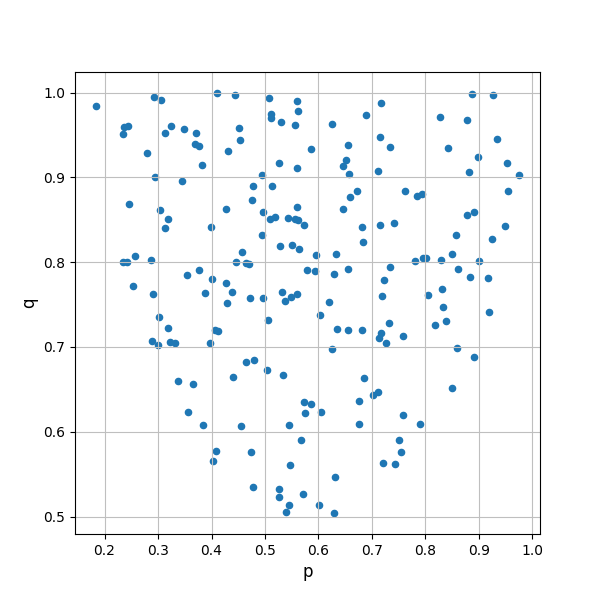
\includegraphics[width=0.5\textwidth]{figures/knuth_die_trueparams.png}
            \label{fig:knuth-die-pq-trueparams}
            \caption{Samples of $(p*,q*)$ that instantiate $\mathcal{M}_{(p*,q*)} \models \Phi$.}
      \end{figure}
\end{example}

\subsection{Summary}
This chapter introduced the essential theoretical concepts of discrete-time models, probabilistic
temporal logic, and parameter synthesis. In the next chapter, we present Bayesian inference methods
for later construction of data-informed parameter synthesis frameworks.